\section{Power/fifth chords}

The power chord, or more formally called a fifth chord, is chord where you only the root and the perfect 5th from that root. You can have multiple octaves of the root and/or fifth in the same chord.

Power chords don't have the 3rd, meaning that they are neither major of minor.

Power chords are often used on electric guitar with distortion. If you would play the full chord (with the 3rd), it can sound quite muddy depending on the amount of distortion.

% https://www.hooktheory.com/blog/power-chords/

\subsection{Notation}
A power chord can be indicated by (taking C and the base):

\begin{itemize}
	\item C5
	\item C(no 3)
\end{itemize}

Both indicate that the power chord doesn't contain the 3rd.

\subsection{Example}

\begin{figure}[h]
	\centering
	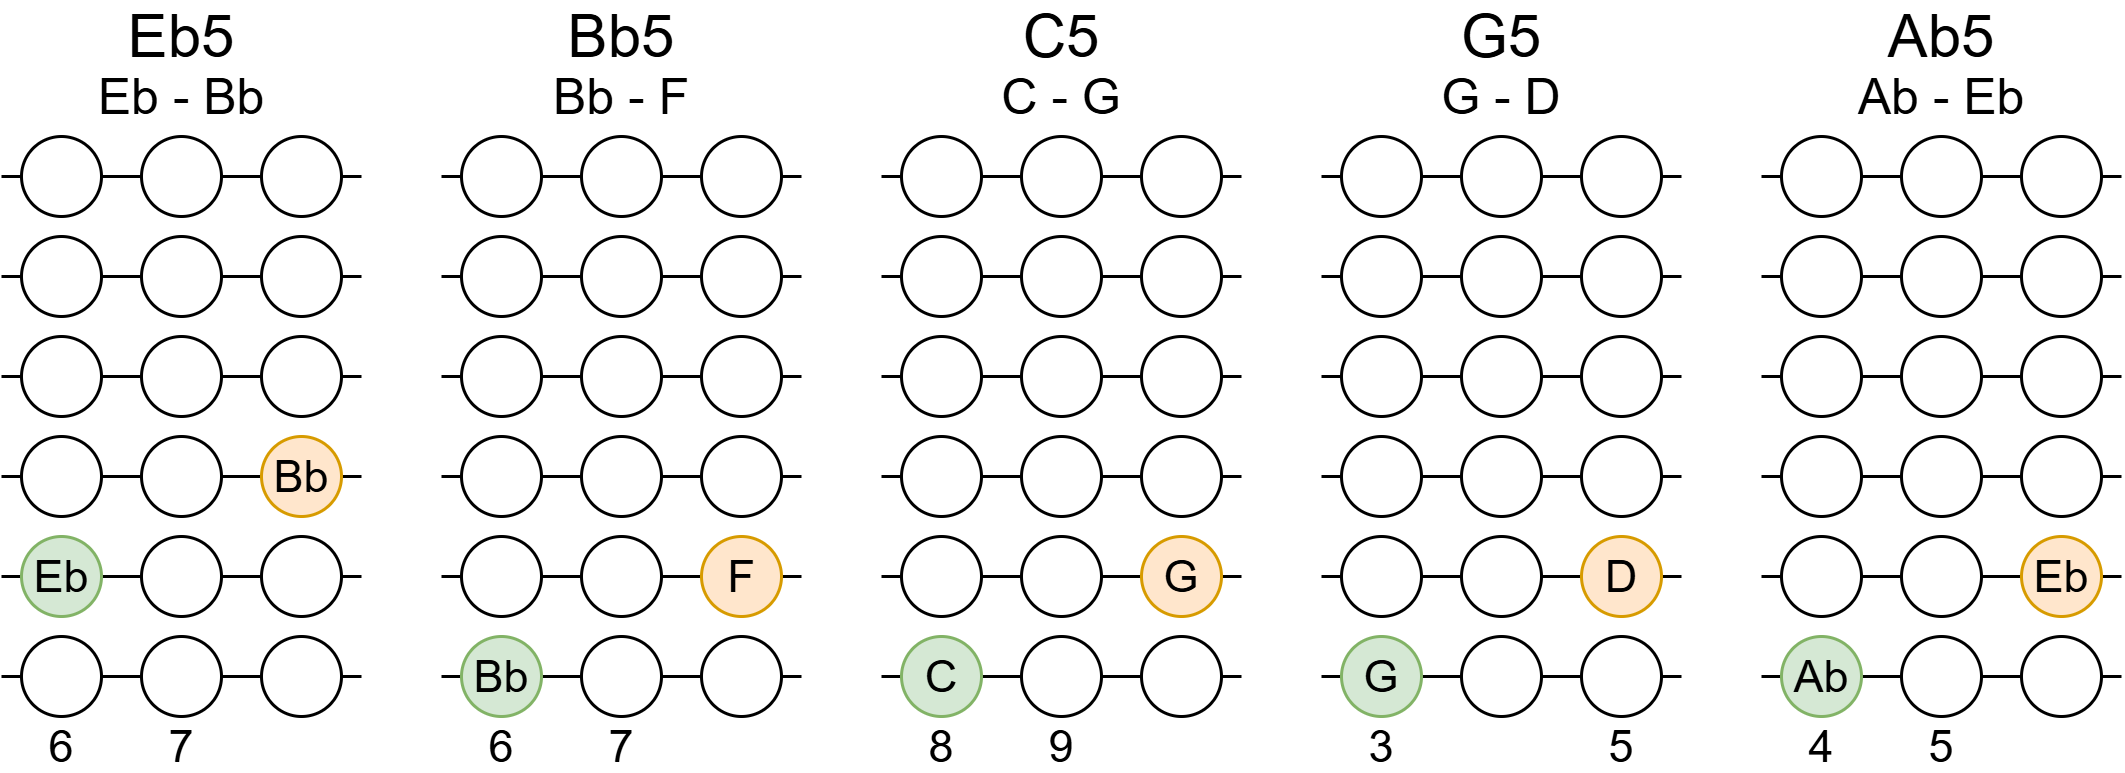
\includegraphics[height=0.16\textheight]{../../Images/ChordsUsedInBasketCaseGreenDayVerse1.png}
	\caption{Chords used in verse 1 of "Basket Case - Green Day"}
	\label{fig:guitar_chords_verse_1_basket_case_green_day}
\end{figure}

Note that on most places on the internet you will find just the chord names without the "5" or "(no 3)". In those cases you have to listen to the song to know what kind of chord is being played. In most cases, for punk, rock, metal, etc. kind of songs, powers chords are a safe bet.

\begin{song}[verse/numbered, align-chords=l]{title={Basket Case - Green Day (verse 1)}, music={Green Day}}
	\begin{verse}
		^{E$\flat$5}Do you have the ^{B$\flat$5}time to ^{C5}listen to me ^{G5}whine? \\
		^{A$\flat$5}About nothing and ^{E$\flat$5}everything, all ^{B$\flat$5}at once \\
		^{E$\flat$5}I am one of ^{B$\flat$5}those ^{C5}melodramatic ^{G5}fools \\
		^{A$\flat$5}Neurotic to the ^{E$\flat$5}bone, no doubt about ^{B$\flat$5}it \\
	\end{verse}
\end{song}

\newpage

\section{Chord inversions}
TODO

\newpage

\section{Diminished \& augmented chords}

Diminished and augmented chords have sort of an uneasy tone. This makes them great as a passing chord to bring in some tension.

Where major and minor chords are identified by their 3rd note, diminished and augmented chords are identified by their 5th note.

Simply put:

\begin{itemize}
	\item \textbf{Diminished} chord: \textbf{minor} chord with the \textbf{5th lowered} by a half step (1 semitone)
	\item \textbf{Augmented} chord: \textbf{major} chord with the \textbf{5th raised} by a half step (1 semitone)
\end{itemize}

\autoref{tab:guitar_diminished_intervals} and \autoref{tab:guitar_augmented_intervals} show how these relate to the major and minor scales (and chords created from them).

\begin{table}[h]
	\centering
	\begin{tabular}{*{17}{c}}
		& & \multicolumn{2}{P{4mm}}{\large{W}} & \multicolumn{2}{P{4mm}}{\large{H}} & \multicolumn{2}{P{4mm}}{\large{W}} & \multicolumn{2}{P{4mm}}{\large{W}} & \multicolumn{2}{P{4mm}}{\large{H}} & \multicolumn{2}{P{4mm}}{\large{W}} & \multicolumn{2}{P{4mm}}{\large{W}} & \\
		Minor intervals & \multicolumn{2}{P{4mm}}{\ScaleRootCellFill 1} & \multicolumn{2}{P{4mm}}{2} & \multicolumn{2}{P{4mm}}{\ScaleCellFill 3$\flat$} & \multicolumn{2}{P{4mm}}{4} & \multicolumn{2}{P{4mm}}{\ScaleCellFill 5} & \multicolumn{2}{P{4mm}}{6$\flat$} & \multicolumn{2}{P{4mm}}{7$\flat$} & \multicolumn{2}{P{4mm}}{8} \\
		Diminished chord from minor scale & \multicolumn{2}{P{4mm}}{\ScaleRootCellFill 1} & \multicolumn{2}{P{4mm}}{} & \multicolumn{2}{P{4mm}}{\ScaleCellFill 3$\flat$} & & \multicolumn{2}{P{4mm}}{\ScaleCellFill 5$\flat$} & & \multicolumn{2}{P{4mm}}{} & \multicolumn{2}{P{4mm}}{} & \multicolumn{2}{P{4mm}}{}
	\end{tabular}
	\caption{Diminished intervals}
	\label{tab:guitar_diminished_intervals}
\end{table}

\begin{table}[h]
	\centering
	\begin{tabular}{*{17}{c}}
		& & \multicolumn{2}{P{4mm}}{\large{W}} & \multicolumn{2}{P{4mm}}{\large{W}} & \multicolumn{2}{P{4mm}}{\large{H}} & \multicolumn{2}{P{4mm}}{\large{W}} & \multicolumn{2}{P{4mm}}{\large{W}} & \multicolumn{2}{P{4mm}}{\large{W}} & \multicolumn{2}{P{4mm}}{\large{H}} & \\
		Major intervals & \multicolumn{2}{P{4mm}}{\ScaleRootCellFill 1} & \multicolumn{2}{P{4mm}}{2} & \multicolumn{2}{P{4mm}}{\ScaleCellFill 3} & \multicolumn{2}{P{4mm}}{4} & \multicolumn{2}{P{4mm}}{\ScaleCellFill 5} & \multicolumn{2}{P{4mm}}{6} & \multicolumn{2}{P{4mm}}{7} & \multicolumn{2}{P{4mm}}{8} \\
		Augmented chord from major scale & \multicolumn{2}{P{4mm}}{\ScaleRootCellFill 1} & \multicolumn{2}{P{4mm}}{} & \multicolumn{2}{P{4mm}}{\ScaleCellFill 3} & \multicolumn{2}{P{4mm}}{} & & \multicolumn{2}{P{4mm}}{\ScaleCellFill 5$\sharp$} & & \multicolumn{2}{P{4mm}}{} & \multicolumn{2}{P{4mm}}{}
	\end{tabular}
	\caption{Augmented intervals}
	\label{tab:guitar_augmented_intervals}
\end{table}

In \autoref{sec:building_chords_with_diatonic_scale} you have already learned the following:

\begin{minipage}{0.5\textwidth}
	\begin{itemize}
		\item Minor chord: 1 - 3$\flat$ - 5:
			\subitem Interval 1 - 3$\flat$: minor 3rd
			\subitem Interval 3$\flat$ - 5: major 3rd
	\end{itemize}
\end{minipage}
\hfill
\begin{minipage}{0.5\textwidth}
	\begin{itemize}
		\item Major chord: 1 - 3 - 5:
			\subitem Interval 1 - 3: major 3rd
			\subitem Interval 3 - 5: minor 3rd
	\end{itemize}
\end{minipage}

Note that both the major and minor chords have a major and minor 3rd stacked on top of each other. Diminished chords have only minor thirds stacked and augmented chords have only major thirds stacked:

\begin{minipage}{0.5\textwidth}
	\begin{itemize}
		\item Diminished chord: 1 - 3$\flat$ - 5$\flat$:
			\subitem Interval 1 - 3$\flat$: minor 3rd
			\subitem Interval 3$\flat$ - 5$\flat$: minor 3rd
	\end{itemize}
\end{minipage}
\hfill
\begin{minipage}{0.5\textwidth}
	\begin{itemize}
		\item Augmented chord: 1 - 3 - 5$\sharp$:
			\subitem Interval 1 - 3: major 3rd
			\subitem Interval 3 - 5$\sharp$: major 3rd
	\end{itemize}
\end{minipage}

Earlier in this book at \autoref{sec:identifying_dimished_chords_in_the_scale} it was explained that a dimished chord has a tritone (meaning 6 semitones). This is the result of stacking two minor 3rd intervals.

% TODO: inversions

\subsection{Notation}
\begin{minipage}{0.4\textwidth}
	Diminished chords can be indicated by (taking C and the base):
	
	\begin{itemize}
		\item Cdim
		\item C($\flat$5)
		\item C\textsuperscript{o}
	\end{itemize}
\end{minipage}
\hfill
\begin{minipage}{0.4\textwidth}
	Augmented chords can be indicated by (taking C and the base):
	
	\begin{itemize}
		\item Caug
		\item C($\sharp$5)
		\item C+
	\end{itemize}
\end{minipage}

\newpage

\subsection{Examples}

% Diminished allstart + don't look back in anger - oasis

The song "All Stars" by "Smash Mouth" uses the diminished chord to bring in some tension.
 
\begin{figure}[h]
	\centering
	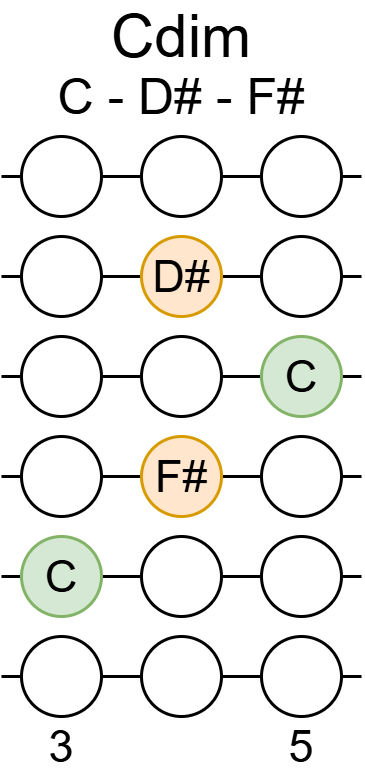
\includegraphics[height=0.16\textheight]{../../Images/CDimChord.png}
	\caption{C$\sharp$dim chord}
	\label{fig:guitar_c_sharp_dim_chord}
\end{figure}

\begin{song}[verse/numbered, align-chords=l]{title={All Stars - Smash Mouth (chorus)}, music={Smash Mouth}}
	\begin{chorus}
		^{F#}Hey now you're an ^{B}All Star get your ^{Cdim}game on, go ^{B}play \\
		^{F#}Hey now you're a ^{B}Rock Star get the ^{Cdim}show on get ^{B}paid \\
		And ^{F#}all that ^{B}glitters is ^{Cdim}gold \\
	 	^{B}Only shooting ^{F#}stars ^{E}break the ^{B}mold \\
	\end{chorus}
\end{song}


% Augmented Impossible Year Chords by Panic! At the Disco
% Augmented Stairway to heaven
% Augmented Life on mars - david bowie

The song "Impossible Year" by "Panic! At The Disco" uses augmented chords to create what is called a "line cliché". This is when either the root of the 5th of a chord is moved up (or down) a semitone a couple of times while keeping the rest of the notes the same. You see that happening here with the 5th of the F chord (see \autoref{fig:guitar_chords_used_in_impossible_year_panic_at_the_disco}).

\begin{figure}[h]
	\centering
	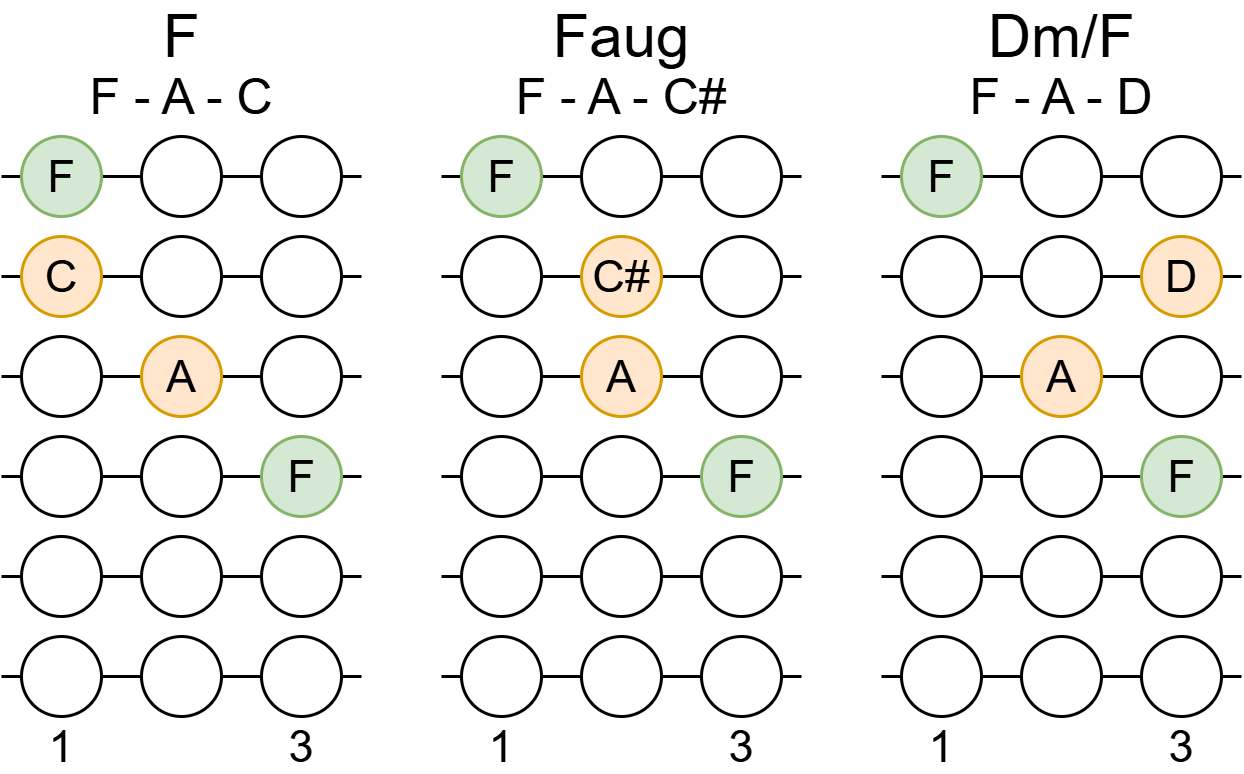
\includegraphics[height=0.16\textheight]{../../Images/ChordsUsedInImpossibleYearPanicAtTheDisco.png}
	\caption{Some of the chords used in "Impossible Year - Panic! At The Disco"}
	\label{fig:guitar_chords_used_in_impossible_year_panic_at_the_disco}
\end{figure}

\begin{song}[verse/numbered, align-chords=l]{title={Impossible Year - Panic! At The Disco (Part of Verse 1)}, music={Panic! At The Disco}}
	\begin{chorus}
		^{F}There's no sunshine ^{Faug} \\
		This ^{Dm/F}impossible year ^{Faug} \\
	\end{chorus}
\end{song}

\newpage

\section{7th chords}
TODO

\newpage

\section{Suspended (sus) chords}
TODO

\newpage

\section{Extended \& Add chords}
TODO
